%
% 公立はこだて未来大学卒業研究中間報告書[全コース対応版]
%
%         ファイル名:"sample.tex"
%
\documentclass[11pt]{jarticle}
\usepackage{funinfosys}
\usepackage{url}
\usepackage[dvipdfmx]{graphicx}
\author{% 
b10xxxxx 未来太郎\\指導教員 : 函館一郎
}
\course{Information Systems Course}
%\course{Advanced ICT Course} %% 高度ICTコースの場合はこちらを使用
%\course{Information Design Course} %% 情報デザインコースの場合はこちらを使用
%\course{Complex Systems Course} %% 複雑系科学コースの場合はこちらを使用
%\course{Intelligent Systems Course} %% 知能システムコースの場合はこちらを使用
\title{中間報告書の書き方}
\etitle{How to Write Manuscripts for Midterm Report}
\eauthor{Taro MIRAI}
\abstract{和文は300から400文字で記述すること.}
\keywords{北海道, 函館, 亀田中野, 公立はこだて未来大学}
\eabstract{English should be written in 100 to 150 words.}
\ekeywords{Hokkaido, Hakodate, Kamedanakano, FUN}
\begin{document}
\maketitle
%\vspace*{-.5cm}

% 背景と目的
\section{背景と目的}

このサンプルは情報システムコースにおける中間報告書の様式について説明したものである.必ずしもこの雛形を使う必要はないが,仕上がりイメージはできる限りこの雛形にあわせること.

用紙サイズはA4,向きは縦とし,上下の余白は30mm、左右の余白は25mmとする.本文には明朝体とTimes New Romanを用いる.ただし,タイトルや章節の見出し,図表のキャプションはゴシック体とする.タイトルは14ポイント,氏名と章の見出しは12ポイント,節の見出しは11ポイント,その他は10ポイントとする.また,和文タイトルから英文キーワードまでは1段,本文は2段で構成とし,1段のセクションは42文字×45行,2段のセクションは20文字×45行とする.

なお,章立てはあくまでも参考であり,\cite{dqn}これに限らない

% 研究の位置づけ
\section{◯◯コースにおける本研究の位置づけ}
中間報告書中のいずれかの場所に,学生所属コースのカリキュラム・ポリシーに基づき,本研究の位置づけを述べる.

未来大学のカリキュラム・ポリシー
\url{https://www.fun.ac.jp/department/curriculum_policy/} のうち,学生所属コースの項に書かれている卒業研究に関する記述を参照.

% 関連研究
\section{関連研究}

中間報告書の文量は4ページとする.学籍番号をファイル名としたPDFファイル1つにまとめた形で作成すること.提出するファイル名はb10xxxxx.pdfとする.

句読点は「,」,「.」とする.「、」,「。」は使用しない.アブストラクトなど英文表記の部分については,スペルチェックプログラムによるチェックをする.


% 提案する理論
\section{提案する理論}

\subsection{数式}

数式による記述が必要な場合は,式番号を適切に参照しながらまとめること.

\subsection{図・写真}

読者の理解を助けるため,図や表を効果的に利用すること.図のキャプションは

\begin{figure}
    \centering
    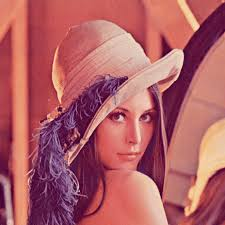
\includegraphics[width=5cm]{figures/Lena.png}
    \caption{This is the most fomous lady. The original image is noode photo.}
\end{figure}

のように,図の下に記す.表のキャプションは

\begin{center}表1 ○○○○\end{center}

のように,表の上に記す.

% 実験と評価
\section{実験と評価}
\par
XXXなを先行研究\cite{rubikcube}と比較する.

% 考察
\section{考察}
\par
僕の考えた最強のネットワーク.

% 結言
\section{結言}
\par
これらの実験から,この研究が最強.

% 参考文献
\bibliography{ref}
\bibliographystyle{junsrt}

\end{document}
%
%
% EOF 
